\labeledsection{Artificial Neural Networks}{sec:ann}
\anondefinition{
An \defemph{Artificial Neural Network (ANN)} is a \linkterm{directed graph}{directed_graph} such that every \linkterm{edge}{undirected_graph} $a_i \to a_j$ is associated with a \defemph{weight} $w_{i,j} \in \mathbb{R}$, and each \linkterm{node}{undirected_graph} $a_j$ with \linkterm{parents}{tree} $a_1, \cdots, a_n$ is associated with a \linkterm{function}{function} $f(w_{1, j}, \cdots w_{n, j}, x_1, \cdots x_n) \in \mathbb{R}$. We call the output of a \linkterm{node}{undirected_graph}'s \linkterm{function}{function} its \defemph{activation}, the matrix $w_{i,j}$ the \defemph{weight matrix}, the \linkterm{nodes}{undirected_graph} \defemph{units} and the \linkterm{edges}{undirected_graph} \defemph{links}
}{ann}

\anondefinition{
A \defemph{McCulloch-Pitts Unit} first computes a weighted sum of all inputs and then applies an \linkterm{activation function}{ann} $g$ to it.
}{mcculloch_pitts}

\anondefinition{
Given a \linkterm{McCulloch-Pitts Unit}{mcculloch_pitts} with an \linkterm{activation function}{ann} $g$. If $g$ is a \linkterm{threshold function}{step_function}, we call the \linkterm{McCulloch-Pitts Unit}{mcculloch_pitts} a \defemph{perceptron unit}, if $g$ is a \linkterm{logistic function}{sigmoid_function}, a \defemph{sigmoid perceptron unit}. 
}{perceptron_sigmoid_unit}

\anondefinition{
A \defemph{McCulloch-Pitts Network} is an \linkterm{Artificial Neural Network}{ann} with \linkterm{McCulloch-Pitts units}{mcculloch_pitts}
}{mcculloch_pitts_network}

\commandnote{
A \linkterm{McCulloch-Pitts Unit}{mcculloch_pitts} computes a linear pre-activation (for example $\mathbf{w}^T\mathbf{x}$). If its activation $g$ is the \linkterm{Heaviside step function}{step_function} the unit implements the \linkterm{Perceptron}{perceptron_hypothesis} — a hard linear classifier trained with the \linkterm{Perceptron Learning Rule}{perceptron_learning_rule}. If $g$ is the \linkterm{logistic function}{sigmoid_function} the unit computes $\sigma(\mathbf{w}^T\mathbf{x})$ and produces a smooth, probability-like score; optimized via gradient-based methods this is the \linkterm{Logistic Regression}{logistic_regression_hypothesis} described in \Secref{sec:regression}. Thus the same McCulloch-Pitts structure with different choices of $g$ connects the perceptron and logistic perspectives: the step activation gives a deterministic decision, while the sigmoid gives a smooth probabilistic output whose $0.5$ threshold recovers the same \linkterm{decision boundary}{decision_boundary} ($\mathbf{w}^T\mathbf{x}=0$).
}

\Example{
We can represent the \texttt{AND} Boolean function as a \linkterm{McCulloch-Pitts Unit}{mcculloch_pitts} with \linkterm{activation function}{ann} $g(r) = 1$ iff $r > 0$, else $0$ (\linkterm{threshold function}{step_function}).

Identify $\texttt{T}=1$ and $\texttt{F}=0$. For inputs $(x_1, x_2) \in \cartprod{\{0,1\}, \{0,1\}}$, choose $x_0=1$ as the dummy input, $w_0=-1$, and $w_1=w_2=1$. Then the weighted sum is
\[
r = w_0x_0 + w_1x_1 + w_2x_2 = -1 + x_1 + x_2.
\]
Now evaluate all four cases:
\[
\begin{array}{c|c|c|c}
x_1 & x_2 & r = -1 + x_1 + x_2 & g(r) \\
\hline
0 & 0 & -1 & 0 \\
0 & 1 & 0 & 0 \\
1 & 0 & 0 & 0 \\
1 & 1 & 1 & 1
\end{array}
\]
So the unit outputs $1$ exactly when both inputs are $1$, which is precisely the \texttt{AND} function.
}{}

\Example{
We can represent the \texttt{OR} Boolean function with the same \linkterm{McCulloch-Pitts Unit}{mcculloch_pitts} setup, again using \linkterm{activation function}{ann} $g(r) = 1$ iff $r > 0$, else $0$ (\linkterm{threshold function}{step_function}).

Identify $\texttt{T}=1$ and $\texttt{F}=0$. For inputs $(x_1, x_2) \in \cartprod{\{0,1\}, \{0,1\}}$, keep $x_0=1$ and $w_1=w_2=1$, but change the bias weight to $w_0=-0.5$. Then the weighted sum is
\[
r = w_0x_0 + w_1x_1 + w_2x_2 = -0.5 + x_1 + x_2.
\]
Now evaluate all four cases:
\[
\begin{array}{c|c|c|c}
x_1 & x_2 & r = -0.5 + x_1 + x_2 & g(r) \\
\hline

0 & 0 & -0.5 & 0 \\
0 & 1 & 0.5 & 1 \\
1 & 0 & 0.5 & 1 \\
1 & 1 & 1.5 & 1
\end{array}
\]
So the unit outputs $1$ whenever at least one input is $1$, which is precisely the \texttt{OR} function.
}{}

\Example{
We can represent the \texttt{NOT} Boolean function with a single-input \linkterm{McCulloch-Pitts Unit}{mcculloch_pitts}, still using \linkterm{activation function}{ann} $g(r) = 1$ iff $r > 0$, else $0$ (\linkterm{threshold function}{step_function}).

Identify $\texttt{T}=1$ and $\texttt{F}=0$. For input $x_1 \in \{0,1\}$, keep $x_0=1$, choose $w_0=0.5$, and choose $w_1=-1$. Then the weighted sum is
\[
r = w_0x_0 + w_1x_1 = 0.5 - x_1.
\]
Now evaluate both cases:
\[
\begin{array}{c|c|c}
x_1 & r = 0.5 - x_1 & g(r) \\
\hline
0 & 0.5 & 1 \\
1 & -0.5 & 0
\end{array}
\]
So the unit outputs $1$ exactly when the input is $0$, which is precisely the \texttt{NOT} function.
}{}

\begin{figure}[H]
    \centering
    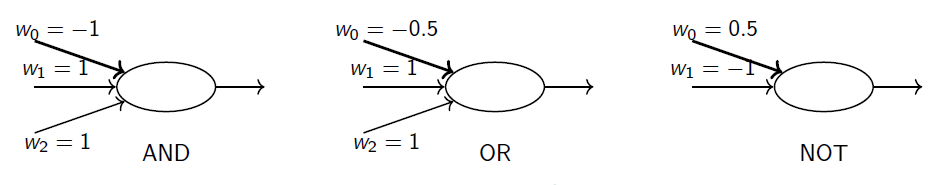
\includegraphics[width=0.5\linewidth]{images/and_or_not.png}
\end{figure}

\observationbox{
By stacking \linkterm{McCulloch-Pitts units}{mcculloch_pitts} into a \linkterm{McCulloch-Pitts Network}{mcculloch_pitts_network}, we can combine simple thresholded units into a larger computation. In particular, since any Boolean function can be written using combinations of \texttt{AND}, \texttt{OR}, and \texttt{NOT}, a finite network of \linkterm{threshold function}{step_function} units can implement any Boolean function on finitely many binary inputs.
}


\Theorem{
Every Boolean function on finitely many binary inputs can be implemented as a \linkterm{McCulloch-Pitts Network}{mcculloch_pitts_network}
}{}

\Example{
The \texttt{XOR} function
\[
x_1 \oplus x_2 = (x_1 \lor x_2) \land \neg (x_1 \land x_2)
\]
can be built from a small \linkterm{McCulloch-Pitts Network}{mcculloch_pitts_network}:

\begin{figure}[H]
    \centering
    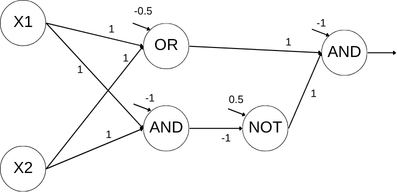
\includegraphics[width=0.3\linewidth]{images/xor_unitsnetwork.png}
\end{figure}
}{}


\anondefinition{
A \linkterm{Neural Network}{ann} is called a \defemph{Feed-Forward Neural Network}, if it is \linkterm{acyclic}{cyclic_graphs}
}{ffnn}

\anondefinition{
A \defemph{perceptron network} is a \linkterm{Feed-Forward Neural Network}{ffnn} of \linkterm{perceptron units}{mcculloch_pitts} (\linkterm{threshold}{step_function}-\linkterm{activated}{ann} \linkterm{McCulloch‑Pitts units}{mcculloch_pitts} ).
}{perceptron_network}

\anondefinition{
\linkterm{Feed-Forward Neural Networks}{ffnn} are usually organized in \defemph{layers}: a \defemph{$n$ layer network} has a partition $\set{L_0, \cdots, L_n}$ of the \linkterm{nodes}{undirected_graph}, such that \linkterm{edges}{undirected_graph} only connect \linkterm{nodes}{undirected_graph} from subsequent \defemph{layer}. $L_0$ is called the \defemph{input layer} and its members \defemph{input units}, and $L_n$ the \defemph{output layer} and its members \defemph{output units}. Any \defemph{unit} that is not in the \defemph{input layer} or the \defemph{output layer} is called \defemph{hidden}
}{layers_neural_nets}

\anondefinition{
A single-\linkterm{layer}{layers_neural_nets} \linkterm{perceptron network}{perceptron_network} is called a \defemph{perceptron}
}{perceptron_nn}

\Example{
\begin{figure}[H]
    \centering
    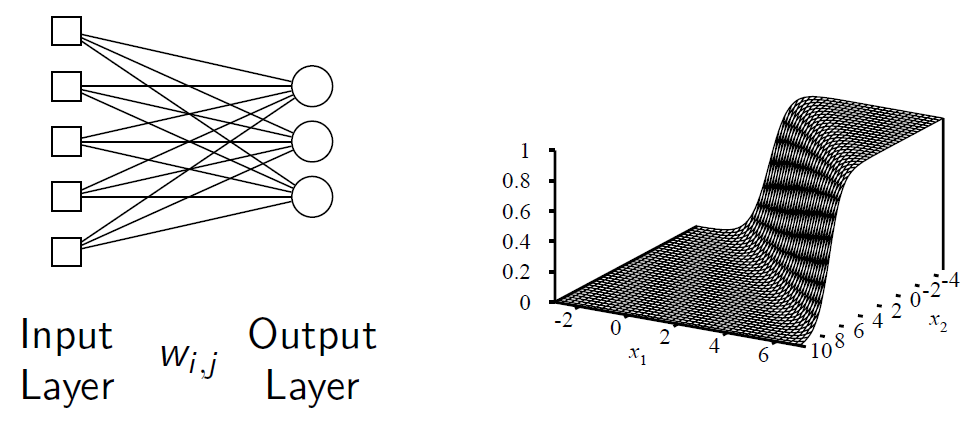
\includegraphics[width=0.3\linewidth]{images/perceptron.png}
\end{figure}
}{}

\titledbox{Expressivity of Perceptrons}{
\linkterm{Perceptrons}{perceptron_nn} can represent \texttt{AND}, \texttt{OR}, \texttt{NOT}, etc. but not \texttt{XOR}. They represent \linkterm{linear separator}{decision_boundary} in input space
}

\begin{figure}[H]
    \centering
    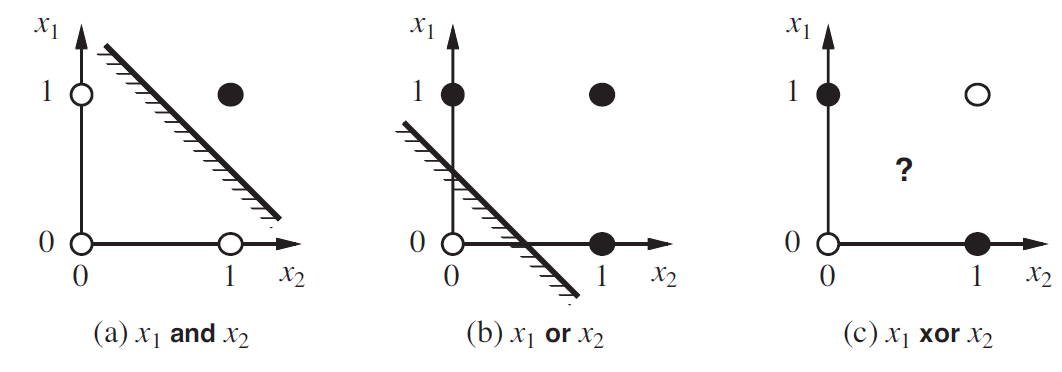
\includegraphics[width=0.5\linewidth]{images/no_xor.png}
\end{figure}

\questionbox{
How \linkterm{perceptrons}{perceptron_nn} learn? (how we update the weights?)
}

\answerbox{
Recall the \linkterm{perceptron learning rule}{perceptron_learning_rule} for \linkterm{multivariate linear regression}{multivariate_linear_regression}.

Single-output (vector form). Let $\mathbf{x}^{(i)}\in\mathbb{R}^{n+1}$ include the bias coordinate $x_0=1$, label $y^{(i)}\in\{0,1\}$, and prediction $\hat{y}^{(i)}=\mathcal{T}(\mathbf{w}^T\mathbf{x}^{(i)})$. The online perceptron update is:
\[
\mathbf{w}^{(t+1)} := \mathbf{w}^{(t)} + \alpha\big(y^{(i)} - \hat{y}^{(i)}\big)\,\mathbf{x}^{(i)}.
\]

Multi-output (single-layer) perceptron. For $K$ output units use a weight matrix $W = (w_{j,k})$, where $j$ indexes the input node and $k$ indexes the output unit. In other words, $w_{j,k}$ is the weight on the edge from the $j$th input unit to the $k$th output unit, and for a fixed $k$ the vector $\mathbf{w}_k = (w_{0,k}, w_{1,k}, \cdots, w_{n,k})^T$ collects all weights feeding into output unit $k$. For each output unit $k$:
\[
\mathbf{w}_k^{(t+1)} := \mathbf{w}_k^{(t)} + \alpha\big(y_k^{(i)} - \hat{y}_k^{(i)}\big)\,\mathbf{x}^{(i)},
\]
or coordinate-wise
\[
w_{j,k}^{(t+1)} := w_{j,k}^{(t)} + \alpha\big(y_k^{(i)} - \hat{y}_k^{(i)}\big) x_j^{(i)}.
\]
}

\questionbox{
What changes when the activation function is smooth and differentiable instead of a threshold?
}

\answerbox{
If a unit computes
\[
h_{\mathbf{w}}(\mathbf{x}^{(i)}) := g\big(\mathbf{w}^T\mathbf{x}^{(i)}\big),
\]
where $g$ is differentiable, then we can no longer use the hard perceptron rule directly. Instead, we minimize a differentiable loss $L$ by gradient descent:
\[
\mathbf{w}^{(t+1)} := \mathbf{w}^{(t)} - \alpha \nabla L.
\]

For a single coordinate $w_{j,k}$, the chain rule gives:
\[
\frac{\partial L}{\partial w_{j,k}}
=
\frac{\partial L}{\partial h_{\mathbf{w}}(\mathbf{x}^{(i)})}
\cdot g'\big(\mathbf{w}^T\mathbf{x}^{(i)}\big)
\cdot x_j^{(i)}.
\]

If we use the squared error loss $L = \frac{1}{2}\big(y_i - h_{\mathbf{w}}(\mathbf{x}^{(i)})\big)^2$, then the update rule becomes:
\[
w_{j,k}^{(t+1)} := w_{j,k}^{(t)} + \alpha\big(y_i - h_{\mathbf{w}}(\mathbf{x}^{(i)})\big)\, g'\big(\mathbf{w}^T\mathbf{x}^{(i)}\big)\, x_j^{(i)}.
\]
So the only extra factor compared to the perceptron update is the derivative of the activation function, $g'$, evaluated at the weighted sum. Here $j$ names the input node and $k$ names the output unit, so $w_{j,k}$ is the weight on the connection from input $j$ to output $k$.
}

\anondefinition{
In \defemph{Multi-Layer Perceptrons (MLPs)}, \linkterm{layers}{layers_neural_nets} are usually fully connected; number of \linkterm{hidden units}{layers_neural_nets} typically chosen by hand
\begin{figure}[H]
    \centering
    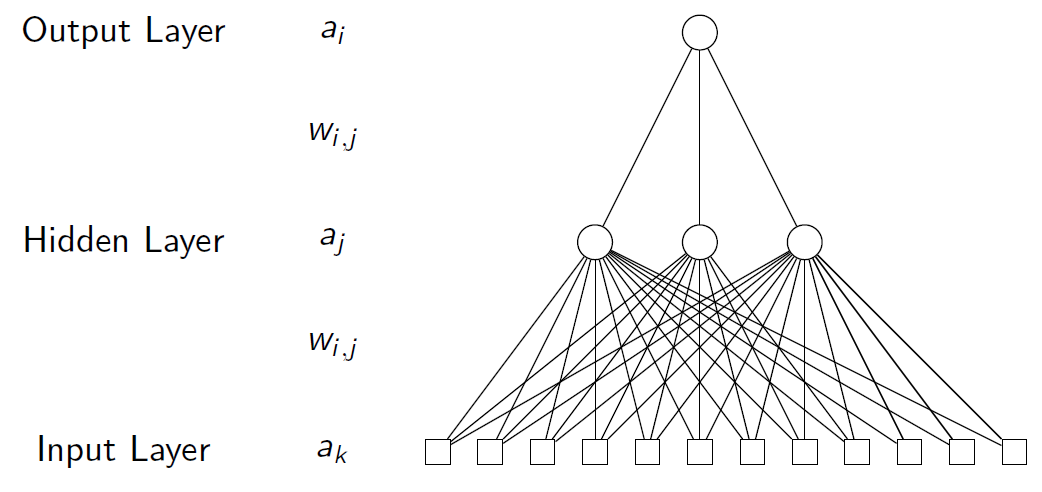
\includegraphics[width=0.3\linewidth]{images/mlp.png}
\end{figure}
}{mlps}

\observationbox{
What we did in the \texttt{XOR} example is actually a \linkterm{MLPs}{mlps}
}

\observationbox{
It allowed us to express a non-linear function (the \texttt{XOR} function)
}

\ideabox{
We can train \linkterm{MLPs}{mlps} on non-linear data! The \linkterm{output layer}{layers_neural_nets} is \linkterm{perceptron}{perceptron_nn} whose input is the output of the last \linkterm{hidden layer}{layers_neural_nets} $\leadsto$ we can use the \linkterm{perceptron learning rule}{perceptron_learning_rule} to update the weights of the \linkterm{output layer}{layers_neural_nets}. 
}

\problembox{
What about the \linkterm{hidden layers}{layers_neural_nets}? We do not have some notion of \textit{"lost / error"} there. How to update the weights ?
}

\ideabox{
The hidden node $j$ is \textit{"responsible"} for some fraction of the error proportional to the weight $w_{j,k}$
}